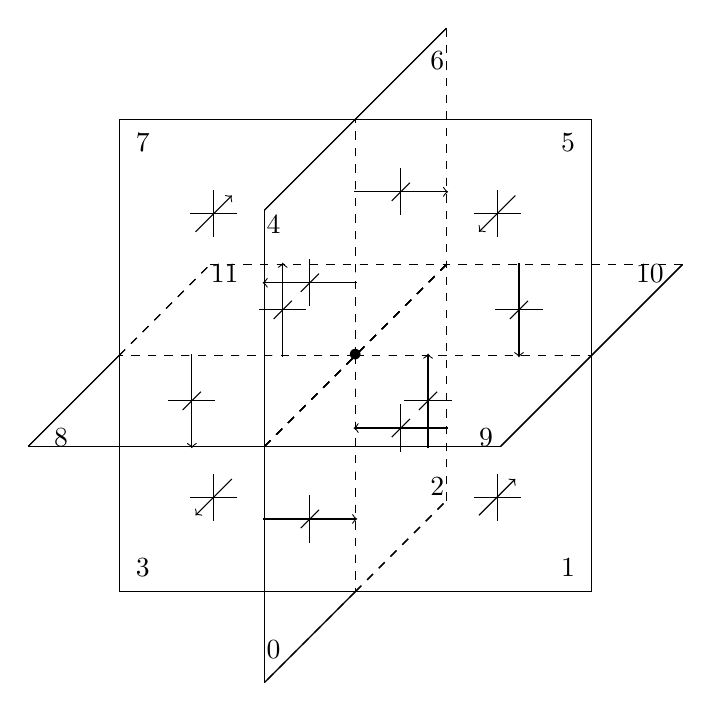
\begin{tikzpicture}[scale = 3, cm={1,0,-1,-1, (0,0)},y=-3.85mm, z = -1cm]


\node at (0,0,0) {$\bullet$};
\node at (0.9,0,-0.9)   {$1$};
\node at (0,0.9,-0.9)   {$2$};
\node at (-0.9,0,-0.9)  {$3$};
\node at (0,-0.9,-0.9)  {$0$};
\node at (0.9,-0.9,0)   {$9$};
\node at (-0.9,-0.9,0)  {$8$};
\node at (-0.9,0.9,0)   {$11$};
\node at (0.9,0.9,0)    {$10$};
\node at (-0.9,0,0.9)   {$7$};
\node at (0.9,0,0.9)    {$5$};
\node at (0,-0.9,0.9)   {$4$};
\node at (0,0.9,0.9)    {$6$};

%Cube Left Front Upper


%Z-Y rectangle X = 0
\draw[] (0,-1,1) -- (0,-1,0);
\draw[dashed] (0,-1,0) -- (0,0,0);
\draw[dashed] (0,0,0)  -- (0,0,1);
\draw[]  (0,0,1) -- (0,-1,1);

%X-Y rectangle Z = 0
\draw[] (-1,-1,0) -- (0,-1,0);
\draw[dashed] (0,-1,0) -- (0,0,0);
\draw[dashed] (0,0,0)  -- (-1,0,0);
\draw[] (-1,0,0) -- (-1,-1,0);

%X-Z rectangle Y = 0
\draw[dashed] (0,0,0)  -- (-1,0,0);
\draw[] (-1,0,0) -- (-1,0,1);
\draw[dashed] (0,0,0)  -- (0,0,1);
\draw[]       (0,0,1)  -- (-1,0,1);



%Cube Right Front Upper

%Y-Z rectangle X = 0
\draw[] (0,-1,1) -- (0,-1,0);
\draw[dashed] (0,-1,0) -- (0,0,0);
\draw[dashed] (0,0,0)  -- (0,0,1);
\draw[]  (0,0,1) -- (0,-1,1);

%X-Y rectangle Z = 0
\draw[] (1,-1,0) -- (0,-1,0);
\draw[dashed] (0,-1,0) -- (0,0,0);
\draw[dashed] (0,0,0)  -- (1,0,0);
\draw[] (1,0,0) -- (1,-1,0);

%X-Z rectangle Y = 0
\draw[dashed] (0,0,0)  -- (1,0,0);
\draw[] (1,0,0) -- (1,0,1);
\draw[dashed] (0,0,0)  -- (0,0,1);
\draw[]       (0,0,1)  -- (1,0,1);



%Cube Right Back Upper

%Y-Z rectangle X = 0
\draw[dashed] (0,1,1) -- (0,1,0);
\draw[dashed] (0,1,0) -- (0,0,0);
\draw[dashed] (0,0,0)  -- (0,0,1);
\draw[]  (0,0,1) -- (0,1,1);

%X-Y rectangle Z = 0
\draw[dashed] (1,1,0) -- (0,1,0);
\draw[dashed] (0,1,0) -- (0,0,0);
\draw[dashed] (0,0,0)  -- (1,0,0);
\draw[] (1,0,0) -- (1,1,0);

%X-Z rectangle Y = 0
\draw[dashed] (0,0,0)  -- (1,0,0);
\draw[] (1,0,0) -- (1,0,1);
\draw[dashed] (0,0,0)  -- (0,0,1);
\draw[]       (0,0,1)  -- (1,0,1);


%Cube Left Back Upper

%Y-Z rectangle X = 0
\draw[dashed] (0,1,1) -- (0,1,0);
\draw[dashed] (0,1,0) -- (0,0,0);
\draw[dashed] (0,0,0)  -- (0,0,1);
\draw[]  (0,0,1) -- (0,1,1);

%X-Y rectangle Z = 0
\draw[dashed] (-1,1,0) -- (0,1,0);
\draw[dashed] (0,1,0) -- (0,0,0);
\draw[dashed] (0,0,0)  -- (-1,0,0);
\draw[dashed] (-1,0,0) -- (-1,1,0);

%X-Z rectangle Y = 0
\draw[dashed] (0,0,0)  -- (-1,0,0);
\draw[dashed] (-1,0,0) -- (-1,0,1);
\draw[dashed] (0,0,0)  -- (0,0,1);
\draw[]       (0,0,1)  -- (-1,0,1);


%Cube Left Front Lower

%Z-Y rectangle X = 0
\draw[] (0,-1,-1) -- (0,-1,0);
\draw[dashed] (0,-1,0) -- (0,0,0);
\draw[dashed] (0,0,0)  -- (0,0,-1);
\draw[]  (0,0,-1) -- (0,-1,-1);

%X-Y rectangle Z = 0
\draw[] (-1,-1,0) -- (0,-1,0);
\draw[dashed] (0,-1,0) -- (0,0,0);
\draw[dashed] (0,0,0)  -- (-1,0,0);
\draw[] (-1,0,0) -- (-1,-1,0);

%X-Z rectangle Y = 0
\draw[dashed] (0,0,0)  -- (-1,0,0);
\draw[] (-1,0,0) -- (-1,0,-1);
\draw[dashed] (0,0,0)  -- (0,0,-1);
\draw[] (0,0,-1)  -- (-1,0,-1);



%Cube Right Front Lower

%Y-Z rectangle X = 0
\draw[] (0,-1,-1) -- (0,-1,0);
\draw[dashed] (0,-1,0) -- (0,0,0);
\draw[dashed] (0,0,0)  -- (0,0,-1);
\draw[dashed]  (0,0,-1) -- (0,-1,-1);

%X-Y rectangle Z = 0
\draw[] (1,-1,0) -- (0,-1,0);
\draw[dashed] (0,-1,0) -- (0,0,0);
\draw[dashed] (0,0,0)  -- (1,0,0);
\draw[] (1,0,0) -- (1,-1,0);

%X-Z rectangle Y = 0
\draw[dashed] (0,0,0)  -- (1,0,0);
\draw[] (1,0,0) -- (1,0,-1);
\draw[dashed] (0,0,0)  -- (0,0,-1);
\draw[] (0,0,-1)  -- (1,0,-1);



%Cube Right Back Lower

%Y-Z rectangle X = 0
\draw[dashed] (0,1,1) -- (0,1,0);
\draw[dashed] (0,1,0) -- (0,0,0);
\draw[dashed] (0,0,0)  -- (0,0,-1);
\draw[dashed]  (0,0,-1) -- (0,1,-1);

%X-Y rectangle Z = 0
\draw[dashed] (1,1,0) -- (0,1,0);
\draw[dashed] (0,1,0) -- (0,0,0);
\draw[dashed] (0,0,0)  -- (1,0,0);
\draw[] (1,0,0) -- (1,1,0);

%X-Z rectangle Y = 0
\draw[dashed] (0,0,0)  -- (1,0,0);
\draw[] (1,0,0) -- (1,0,-1);
\draw[dashed] (0,0,0)  -- (0,0,-1);
\draw[dashed]       (0,0,-1)  -- (1,0,-1);


%Cube Left Back Lower

%Y-Z rectangle X = 0
\draw[dashed] (0,1,-1) -- (0,1,0);
\draw[dashed] (0,1,0) -- (0,0,0);
\draw[dashed] (0,0,0)  -- (0,0,-1);
\draw[dashed]  (0,0,-1) -- (0,1,-1);

%X-Y rectangle Z = 0
\draw[dashed] (-1,1,0) -- (0,1,0);
\draw[dashed] (0,1,0) -- (0,0,0);
\draw[dashed] (0,0,0)  -- (-1,0,0);
\draw[dashed] (-1,0,0) -- (-1,1,0);

%X-Z rectangle Y = 0
\draw[dashed] (0,0,0)  -- (-1,0,0);
\draw[dashed] (-1,0,0) -- (-1,0,-1);
\draw[dashed] (0,0,0)  -- (0,0,-1);
\draw[dashed]       (0,0,-1)  -- (-1,0,-1);


%Arrows
\draw[->] (0.6,-0.2,-0.6) -- (0.6,0.2,-0.6);
\draw[]   (0.5,0,-0.6)    -- (0.7,0,-0.6);
\draw[]   (0.6,0,-0.5)    -- (0.6,0,-0.7);

\draw[<-] (0.2,-0.5,-0.5) -- (-0.2,-0.5,-0.5);
\draw[]   (0,-0.6,-0.5)   -- (0,-0.4,-0.5);
\draw[]   (0,-0.5,-0.6)   -- (0,-0.5,-0.4);

\draw[->] (0.2,0.5,-0.5) -- (-0.2,0.5,-0.5);
\draw[]   (0,0.6,-0.5)   -- (0,0.4,-0.5);
\draw[]   (0,0.5,-0.6)   -- (0,0.5,-0.4);

\draw[<-] (0.6,-0.2,0.6) -- (0.6,0.2,0.6);
\draw[]   (0.5,0,0.6)    -- (0.7,0,0.6);
\draw[]   (0.6,0,0.5)    -- (0.6,0,0.7);

\draw[->] (-0.6,-0.2,0.6) -- (-0.6,0.2,0.6);
\draw[]   (-0.5,0,0.6)    -- (-0.7,0,0.6);
\draw[]   (-0.6,0,0.5)    -- (-0.6,0,0.7);

\draw[<-] (-0.6,-0.2,-0.6) -- (-0.6,0.2,-0.6);
\draw[]   (-0.5,0,-0.6)    -- (-0.7,0,-0.6);
\draw[]   (-0.6,0,-0.5)    -- (-0.6,0,-0.7);

\draw[->] (0.2,-0.5,0.5) -- (-0.2,-0.5,0.5);
\draw[]   (0,-0.6,0.5)   -- (0,-0.4,0.5);
\draw[]   (0,-0.5,0.6)   -- (0,-0.5,0.4);

\draw[<-] (0.2,0.5,0.5) -- (-0.2,0.5,0.5);
\draw[]   (0,0.6,0.5)   -- (0,0.4,0.5);
\draw[]   (0,0.5,0.6)   -- (0,0.5,0.4);

\draw[->] (0.5,-0.5,-0.2) -- (0.5,-0.5,0.2);
\draw[]   (0.6,-0.5,0)    -- (0.4,-0.5,0);
\draw[]   (0.5,-0.4,0)    -- (0.5,-0.6,0);

\draw[<-] (-0.5,-0.5,-0.2) -- (-0.5,-0.5,0.2);
\draw[]   (-0.6,-0.5,0)    -- (-0.4,-0.5,0);
\draw[]   (-0.5,-0.4,0)    -- (-0.5,-0.6,0);

\draw[->] (-0.5,0.5,-0.2) -- (-0.5,0.5,0.2);
\draw[]   (-0.6,0.5,0)    -- (-0.4,0.5,0);
\draw[]   (-0.5,0.4,0)    -- (-0.5,0.6,0);

\draw[<-] (0.5,0.5,-0.2) -- (0.5,0.5,0.2);
\draw[]   (0.6,0.5,0)    -- (0.4,0.5,0);
\draw[]   (0.5,0.4,0)    -- (0.5,0.6,0);


\end{tikzpicture}
